На рисунке \ref{img:pipeline} показана реализация класса Stitcher библиотеки OpenCV, отвечающий за выполнение сшивающего конвейера. Используя этот класс можно управлять этапами выполнения конвейера.

\begin{figure}[h!]
	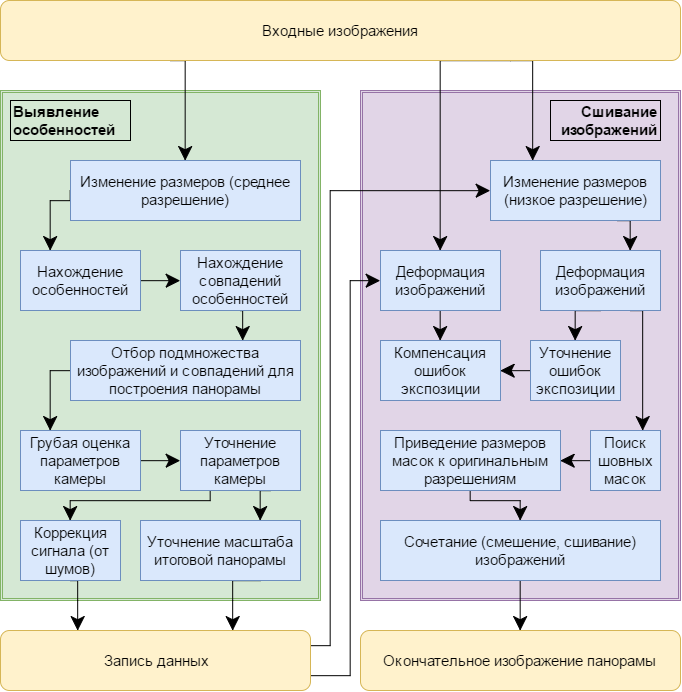
\includegraphics[width = \linewidth]{img/pipeline}
	\caption{схема работы сшивающего контейнера, реализованного в классе Stitcher.}
	\label{img:pipeline}
\end{figure}

Стоит отметить, что это общая последовательность работы класса Stitcher. Данная схема была взята из документации к версии OpenCV 2.4 со ссылкой на статью: Brown and D. Lowe. Automatic Panoramic Image Stitching using Invariant Features. International Journal of Computer Vision, 74(1), страницы 59-73, 2007 года.

В OpenCV 3.2, использовавшемся при выполнении работы, конвейер сохраняется и для построения панорамы выполняются примерно следующие шаги:

\begin{enumerate}
	\item Обнаружение ключевых точек (методы DoG, Harris, и т.д.) и описание локальных ориентиров (при помощи алгоритмов SIFT, SURF, и т.д.) по первым двум изображениям.
	\item Нахождение совпадений описаний ориентиров между двумя изображениями.
	\item \label{it:hom_matrix} Использование алгоритма RANSAC (RANdom SAmple Consensus — стабильный метод оценки параметров модели на основе случайных выборок) для оценки матрицы гомографии используя вектора описаний совпавших ориентиров.
	\item Применение деформирующих преобразований, используя матрицу гомографии, найденную на шаге \ref{it:hom_matrix}.
\end{enumerate}

Основная разница между реализацией Stitcher в OpenCV 2.4 и 3.2 в методах обнаружения ключевых точек и описаний локальных ориентиров (таких как SIFT и SURF).